\chapter{Satuan, Dimensi, dan Pengukuran}\label{ch:b1:units-dimensions}

Di sebuah laboratorium di ruang bawah tanah sebuah bandul berayun,
sebuah stopwatch berdetak, dan seorang mahasiswa menuliskan
$g = \qty{9.77}{m/s^2}$. Apakah itu nilai yang ``benar''? Buku teks
menyebut $9.81$. Apakah kedua angka itu selaras, apakah percobaannya
dirancang dengan baik, langkah mana yang membatasinya --- tidak satu pun
dapat diputuskan dari digitnya saja. Fisika mengukur, dan pengukuran
tanpa ketidakpastiannya hanyalah kabar angin. Bab ini menyiapkan bahasa
bersama bagi seluruh bab berikutnya: \omterm{def:b1:units-dimensions:unit}{satuan}, \omterm{def:b1:units-dimensions:dimension}{dimensi}, \omterm{def:b1:units-dimensions:oom}{orde besar}, dan
aritmetika ketidakpastian yang jujur.

\begin{omfigure}
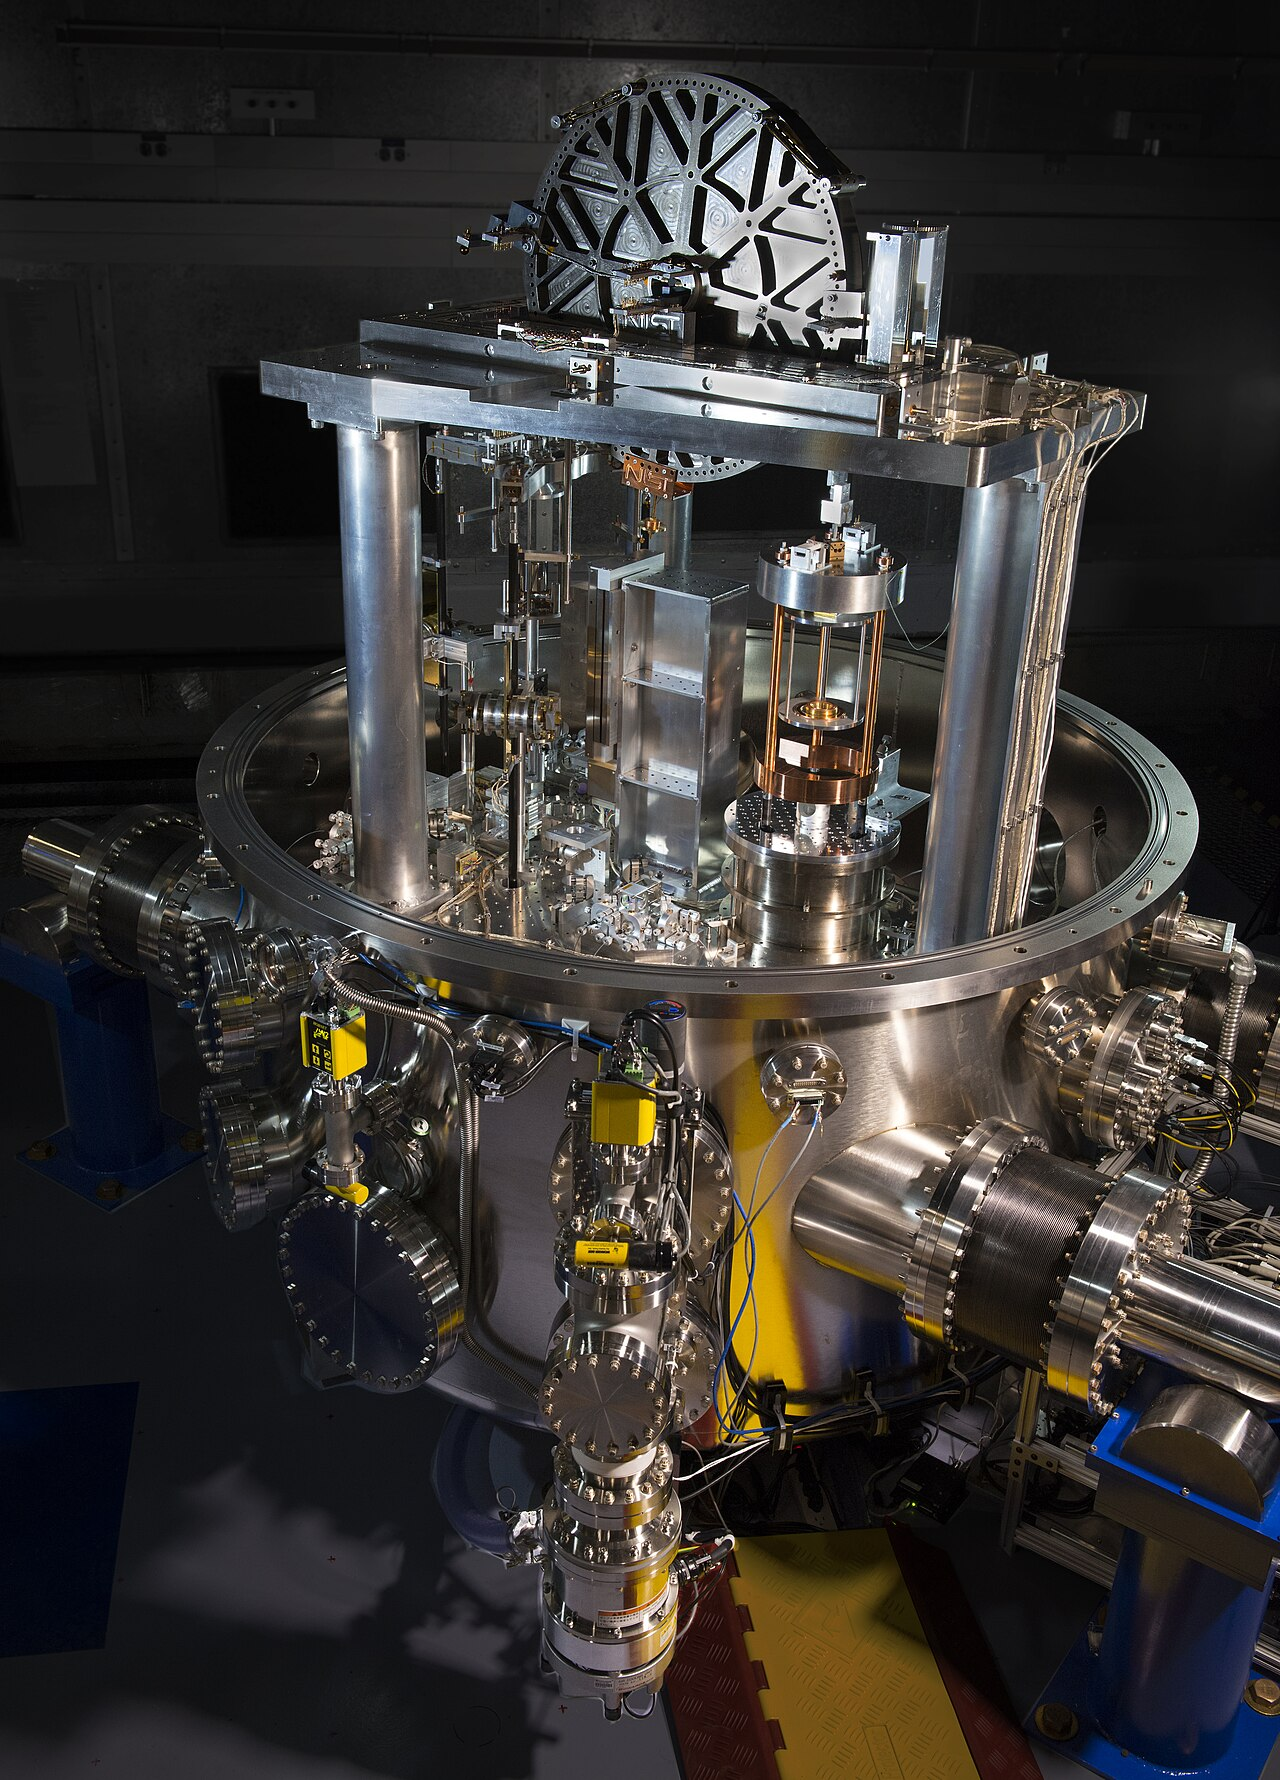
\includegraphics[width=0.46\linewidth]{images/book3/kibble-balance-nist.jpg}

{\small Neraca Kibble NIST-4, salah satu instrumen yang kini mewujudkan kilogram dari tetapan Planck: sebuah massa ditimbang terhadap gaya elektromagnetik yang diukur dalam \omterm{def:b1:units-dimensions:unit}{satuan} listrik. Foto: J.~L.~Lee, NIST (domain publik).}
\end{omfigure}

\section{Sistem Satuan Internasional}

\begin{definition}[Besaran fisis dan satuan]\label{def:b1:units-dimensions:unit}
Sebuah \emph{besaran fisis}\index{besaran fisis} adalah sifat yang
dapat diukur: panjang, selang waktu, massa, arus. Mengukurnya berarti
membandingkannya dengan besaran acuan sejenis, yaitu
\emph{satuan}\index{satuan}: hasilnya sebuah bilangan dikali satuan,
$\ell = \qty{1.257}{m}$. Bilangannya saja tidak berarti apa-apa;
satuannya saja tidak mengukur apa pun.
\end{definition}

\begin{definition}[Satuan dasar SI]\label{def:b1:units-dimensions:si}
\index{SI (Sistem Satuan Internasional)}\index{satuan dasar}
\emph{Sistem \omterm{def:b1:units-dimensions:unit}{Satuan} Internasional} (SI) bertumpu pada tujuh
\emph{\omterm{def:b1:units-dimensions:unit}{satuan} dasar}: sekon (\unit{s}), meter (\unit{m}),
kilogram (\unit{kg}), ampere (\unit{A}), kelvin (\unit{K}),
mol (\unit{mol}) dan candela (\unit{cd}). Sejak 2019 masing-masing
didefinisikan dengan menetapkan nilai numerik sebuah tetapan alam:
frekuensi hiperhalus sesium $\Delta\nu_{\mathrm{Cs}} = \qty{9192631770}{Hz}$
mendefinisikan sekon; laju cahaya $c = \qty{299792458}{m/s}$ lalu
mendefinisikan meter; tetapan Planck
$h = \qty{6.62607015e-34}{J.s}$ mendefinisikan kilogram; muatan
elementer $e = \qty{1.602176634e-19}{C}$ mendefinisikan ampere; tetapan Boltzmann
$k_B = \qty{1.380649e-23}{J/K}$ mendefinisikan kelvin; tetapan Avogadro
$N_A = \qty{6.02214076e23}{mol^{-1}}$ mendefinisikan mol; dan efikasi
cahaya tetap $K_{\mathrm{cd}}$ mendefinisikan candela. Setiap \omterm{def:b1:units-dimensions:unit}{satuan} lain adalah
\emph{satuan turunan}\index{satuan turunan}, hasil kali pangkat-pangkat
\omterm{def:b1:units-dimensions:unit}{satuan} dasar: $\qty{1}{N} = \qty{1}{kg.m/s^2}$, $\qty{1}{J} = \qty{1}{N.m}$,
$\qty{1}{W} = \qty{1}{J/s}$, $\qty{1}{V} = \qty{1}{W/A}$,
$\qty{1}{Pa} = \qty{1}{N/m^2}$.
\end{definition}

\begin{omfigure}
\begin{tikzpicture}[font=\footnotesize, scale=0.95]
  \def\R{3.3} \def\r{1.75}
  \foreach \i/\a/\u/\c in {1/90/{\unit{s}}/{$\Delta\nu_{\mathrm{Cs}}$},
      2/141.4/{\unit{m}}/{$c$}, 3/192.9/{\unit{kg}}/{$h$},
      4/244.3/{\unit{A}}/{$e$}, 5/295.7/{\unit{K}}/{$k_B$},
      6/347.1/{\unit{mol}}/{$N_A$}, 7/38.6/{\unit{cd}}/{$K_{\mathrm{cd}}$}}{
    \node[draw, omDef, thick, circle, minimum size=8.2mm, fill=omDef!8]
      (U\i) at (\a:\R) {\u};
    \node[draw, omThm, circle, minimum size=7.5mm, fill=omThm!6]
      (C\i) at (\a:\r) {\c};
    \draw[-Stealth, omExo] (C\i) -- (U\i);
  }
  \draw[omExo, dashed, -Stealth] (U1) to[bend right=22] (U2);
  \draw[omExo, dashed, -Stealth] (U2) to[bend right=22] (U3);
  \draw[omExo, dashed, -Stealth] (U3) to[bend right=22] (U4);
\end{tikzpicture}

{\small Tujuh \omterm{def:b1:units-dimensions:si}{satuan dasar} (cincin luar) dan tujuh tetapan
pendefinisi (cincin dalam). Sebuah tetapan yang ditetapkan hanya
mendefinisikan \omterm{def:b1:units-dimensions:unit}{satuannya} bersama \omterm{def:b1:units-dimensions:unit}{satuan} yang sudah terdefinisi (garis
putus-putus): $c$ mengubah sekon menjadi meter, $h$ memerlukan meter
dan sekon untuk mendefinisikan kilogram, $e$ memerlukan sekon untuk
mendefinisikan ampere.}
\end{omfigure}

\begin{remark}[Nama dan lambang]\label{rem:b1:units-dimensions:names}
\omterm{def:b1:units-dimensions:unit}{Satuan} yang dinamai menurut nama orang ditulis dengan huruf kecil bila
dieja penuh (newton, joule, pascal) dan dengan huruf besar sebagai
lambang (\unit{N}, \unit{J}, \unit{Pa}); dieja penuh dengan huruf
besar, kata itu berarti orangnya. Awalan menskalakan dengan pangkat
sepuluh, dari p ($10^{-12}$) melalui n, $\mu$, m, k, M, G sampai T
($10^{12}$); kilogram adalah satu-satunya \omterm{def:b1:units-dimensions:si}{satuan dasar} yang membawa
awalan pada namanya.
\end{remark}

\begin{example}[Menguraikan sebuah satuan turunan]\label{ex:b1:units-dimensions:unpack}
Volt: $\unit{V} = \unit{W/A} = \unit{J/(A.s)} = \unit{kg.m^2/(A.s^3)}$.
Ohm: $\unit{\ohm} = \unit{V/A} = \unit{kg.m^2/(A^2.s^3)}$. Farad:
$\unit{F} = \unit{C/V} = \unit{A.s/V} = \unit{A^2.s^4/(kg.m^2)}$.
Penguraian seperti ini adalah pemeriksaan teraman bahwa sebuah rumus
diingat dengan benar --- subbab berikut membuatnya sistematis.
\end{example}

\section{Analisis dimensi}

\begin{definition}[Dimensi]\label{def:b1:units-dimensions:dimension}
\index{dimensi}\index{tak berdimensi}
\emph{Dimensi} sebuah besaran $X$, ditulis $[X]$, mencatat bagaimana
$X$ tersusun dari tujuh besaran dasar, terlepas dari \omterm{def:b1:units-dimensions:unit}{satuan} yang
dipilih: panjang $L$, massa $M$, waktu $T$, arus listrik $I$,
suhu $\Theta$, jumlah zat $N$, intensitas cahaya $J$.
Kelajuan berdimensi $[v] = L\,T^{-1}$, gaya
$[F] = M\,L\,T^{-2}$, energi $[E] = M\,L^2\,T^{-2}$. Besaran
berdimensi $1$ (sudut, nisbah, indeks bias) disebut
\emph{tak berdimensi}.
\end{definition}

\begin{theorem}[Asas kehomogenan dimensi]\label{thm:b1:units-dimensions:homogeneity}
\index{kehomogenan dimensi}
Dalam sebuah hukum fisika, kedua ruas sebuah kesamaan berdimensi sama,
dan setiap suku sebuah penjumlahan berdimensi sama dengan keseluruhannya.
Argumen eksponensial, logaritma, sinus atau kosinus \omterm{def:b1:units-dimensions:dimension}{tak berdimensi}.
\end{theorem}

\begin{proof}
Hukum-hukum fisika tidak bergantung pada \omterm{def:b1:units-dimensions:unit}{satuan} yang dipilih manusia.
Mengubah \omterm{def:b1:units-dimensions:unit}{satuan} panjang dengan faktor $\lambda$ mengalikan setiap
besaran berdimensi $L^a \cdots$ dengan $\lambda^{-a}$: sebuah kesamaan
antara suku-suku berdimensi berbeda akan berlaku dalam satu sistem
\omterm{def:b1:units-dimensions:unit}{satuan} dan gagal dalam sistem yang lain. Untuk fungsi seperti $\exp$,
deret $1 + x + x^2/2 + \dots$ menjumlahkan pangkat-pangkat $x$ yang
berbeda \omterm{def:b1:units-dimensions:dimension}{dimensi} kecuali jika $x$ \omterm{def:b1:units-dimensions:dimension}{tak berdimensi}.
\end{proof}

\begin{method}[Memeriksa sebuah rumus]\label{met:b1:units-dimensions:check}
\begin{enumerate}
  \item Tuliskan \omterm{def:b1:units-dimensions:dimension}{dimensi} setiap lambang.
  \item Sederhanakan tiap ruas (tiap suku) menjadi hasil kali
        $L^a M^b T^c \cdots$.
  \item Pangkat sama pada kedua ruas: rumusnya \emph{mungkin} benar.
        Pangkat berbeda: rumusnya pasti salah --- ada faktor $g$ yang
        hilang, besaran yang dikuadratkan padahal tidak seharusnya,
        atau pangkat yang berdimensi.
\end{enumerate}
Rumus yang homogen masih bisa salah pada faktor \omterm{def:b1:units-dimensions:dimension}{tak berdimensi}
($2$, $\pi$, $\tfrac12$): \omterm{def:b1:units-dimensions:dimension}{dimensi} tidak pernah melihatnya.
\end{method}

\begin{example}[Periode sebuah bandul]\label{ex:b1:units-dimensions:pendulum}
Sebuah bandul sepanjang $\ell$ bermassa $m$ berayun dalam gravitasi
$g$. Andaikan periodenya $\tau = k\,\ell^\alpha m^\beta g^\gamma$
dengan $k$ \omterm{def:b1:units-dimensions:dimension}{tak berdimensi}. Maka $T = L^\alpha M^\beta (L T^{-2})^\gamma =
L^{\alpha+\gamma} M^\beta T^{-2\gamma}$, sehingga $\beta = 0$,
$\gamma = -\tfrac12$, $\alpha = \tfrac12$:
\[
\tau = k\sqrt{\ell/g} .
\]
Tanpa menyelesaikan satu pun persamaan gerak: massanya lenyap, dan
melipatduakan panjangnya mengalikan periodenya dengan $\sqrt2$. Dinamika
(\cref{ch:b1:oscillators-resonance}) kelak memberi $k = 2\pi$ untuk
ayunan kecil.
\end{example}

\begin{proposition}[Kelompok tak berdimensi]\label{prop:b1:units-dimensions:pi}
\index{kelompok tak berdimensi}
Jika sebuah besaran $Y$ bergantung pada $n$ besaran $X_1, \dots, X_n$
yang melibatkan $r$ \omterm{def:b1:units-dimensions:dimension}{dimensi} dasar yang bebas, hubungan itu dapat ditulis
ulang antara $n + 1 - r$ kombinasi \omterm{def:b1:units-dimensions:dimension}{tak berdimensi} dari $X_i$ dan $Y$.
Ketika $n + 1 - r = 1$, kombinasi tunggal itu harus tetap, dan analisis
\omterm{def:b1:units-dimensions:dimension}{dimensi} memberikan hukumnya sampai pada sebuah faktor numerik.
\end{proposition}
\admitted

\begin{remark}[Menggunakan proposisi]\label{rem:b1:units-dimensions:pi}
Pernyataan umumnya (teorema Vaschy--Buckingham) adalah sepotong aljabar
linear atas vektor-vektor pangkat. Yang penting di sini resepnya:
daftarkan besaran yang relevan, hitung \omterm{def:b1:units-dimensions:dimension}{dimensinya}, bentuk \omterm{prop:b1:units-dimensions:pi}{kelompok tak
berdimensinya}. Dalam \cref{ex:b1:units-dimensions:pendulum}, $n = 3$
($\ell, m, g$), $r = 3$ ($L, M, T$), sehingga ada satu kelompok
$\tau\sqrt{g/\ell}$ dan ia harus tetap. Hambatan pada sebuah bola
berjari-jari $R$ yang bergerak dengan laju $v$ dalam fluida bermassa
jenis $\rho$ dan berkekentalan $\eta$ melibatkan $n = 4$ besaran dan
$r = 3$ \omterm{def:b1:units-dimensions:dimension}{dimensi}: dua kelompok, $F/(\rho v^2 R^2)$ dan $\rho v R/\eta$
(bilangan Reynolds), dan \omterm{def:b1:units-dimensions:dimension}{dimensi} saja tidak dapat mengatakan bagaimana
yang pertama bergantung pada yang kedua --- percobaan yang harus.
\end{remark}

\section{Orde besar}

\begin{definition}[Orde besar]\label{def:b1:units-dimensions:oom}
\index{orde besar}
\emph{Orde besar} sebuah besaran adalah pangkat sepuluh yang terdekat
kepadanya: $\qty{6.4e6}{m}$ (jari-jari Bumi) berorde besar
$10^7$; $\qty{3e3}{m}$ berorde $10^3$; $\qty{3.2e3}{m}$ lebih dekat ke
$10^3$ daripada ke $10^4$ pada skala logaritmik (batasnya
$\sqrt{10} \approx 3.16$). Dua besaran disebut ``seorde'' bila
nisbahnya di bawah kira-kira $3$.
\end{definition}

\begin{method}[Menaksir]\label{met:b1:units-dimensions:estimate}
Untuk menaksir besaran yang tidak diukurkan siapa pun untuk Anda:
\begin{enumerate}
  \item uraikan menjadi faktor-faktor yang dapat Anda taksir sampai
        pada faktor $2$ atau $3$ masing-masing;
  \item taksir tiap faktor, pertahankan satu \omterm{def:b1:units-dimensions:sigfig}{angka penting};
  \item kalikan, pertahankan pangkat sepuluh dan satu digit.
\end{enumerate}
Galat pada faktor yang berbeda sebagian saling meniadakan; hasilnya
biasanya benar sampai pada faktor $3$ sampai $10$, yang seringkali
sudah cukup untuk menerima atau menolak sebuah hipotesis.
\end{method}

\begin{example}[Massa atmosfer]\label{ex:b1:units-dimensions:atmosphere}
Tekanan atmosfer $P_0 \approx \qty{1e5}{Pa}$ adalah berat kolom udara
di atas satu meter persegi, $P_0 = m_{\text{kol}}\,g$, sehingga
$m_{\text{kol}} \approx 10^5/10 = \qty{1e4}{kg}$ tiap meter persegi.
Permukaan Bumi seluas $4\pi R^2 \approx 4 \times 3 \times (6\times10^6)^2
\approx \qty{5e14}{m^2}$; jadi atmosfer berbobot sekitar
$\qty{5e18}{kg}$. Nilai yang diterima $\qty{5.1e18}{kg}$ --- taksiran
itu hanya memerlukan $P_0$ dan $R$.
\end{example}

\begin{definition}[Angka penting]\label{def:b1:units-dimensions:sigfig}
\index{angka penting}
\emph{Angka penting} sebuah bilangan tertulis adalah digitnya terhitung
dari yang pertama tak nol: $0.0820$ punya tiga, $\num{8.20e-2}$ punya
tiga yang sama, $820$ bermakna ganda (dua atau tiga) kecuali ditulis
\num{8.2e2} atau \num{8.20e2}. Sebuah hasil ditulis dengan angka
penting sebanyak yang diizinkan ketidakpastiannya
(\cref{met:b1:units-dimensions:writing} di bawah): bukan
``$g = \qty{9.7723}{m/s^2}$'' bila digit keempatnya tak diketahui.
\end{definition}

\section{Ketidakpastian pengukuran}

\begin{definition}[Besaran ukur, galat, ketidakpastian]\label{def:b1:units-dimensions:uncertainty}
\index{besaran ukur}\index{galat pengukuran}\index{ketidakpastian baku}
\emph{Besaran ukur} adalah besaran yang hendak diukur. Mengulang sebuah
pengukuran memberi nilai yang berpencar: pengukurannya bersifat
\emph{beragam}. \emph{Galat} sebuah hasil adalah selisihnya yang tak
diketahui terhadap nilai benar; \emph{ketidakpastian baku} $u(x)$
sebuah hasil $x$ adalah simpangan baku nilai-nilai yang secara masuk
akal dapat dikaitkan dengan besaran ukur --- besaran yang justru
\emph{dapat} dievaluasi. Sumbernya: pengamat (waktu reaksi, paralaks),
lingkungan (suhu, getaran), instrumen (resolusi, kalibrasi), dan
metodenya (model yang hanya hampir benar).
\end{definition}

\begin{proposition}[Evaluasi tipe A]\label{prop:b1:units-dimensions:typeA}
\index{ketidakpastian!tipe A}
Dari $n$ nilai ulangan yang saling bebas $x_1, \dots, x_n$ dengan
rata-rata $\bar x = \frac1n \sum x_i$ dan simpangan baku eksperimen
\[
s = \sqrt{\frac{1}{n-1}\sum_{i=1}^n (x_i - \bar x)^2},
\]
taksiran terbaik \omterm{def:b1:units-dimensions:uncertainty}{besaran ukurnya} adalah $\bar x$ dan \omterm{def:b1:units-dimensions:uncertainty}{ketidakpastian
bakunya}
\[
u(\bar x) = \frac{s}{\sqrt n} .
\]
\end{proposition}

\begin{proof}[Bukti sebagian]
Bahwa $s$ menaksir pencaran satu pengukuran tunggal adalah definisi
simpangan baku eksperimen ($n - 1$ dan bukan $n$ karena rata-ratanya
sendiri ditaksir dari datanya). Bahwa rata-rata $n$ nilai yang saling
bebas berpencar $\sqrt n$ kali lebih sempit daripada satu nilai adalah
penjumlahan ragam: ragam jumlah $n$ peubah yang saling bebas sama
dengan $n$ kali ragam satu peubah, sehingga ragam rata-ratanya
$s^2 n / n^2 = s^2/n$. Kuliah peluang tahun ini membuktikan keduanya.
\end{proof}

\begin{omfigure}
\begin{tikzpicture}
\begin{axis}[omaxis, width=9.6cm, height=5.6cm, xlabel={$T$ (\unit{s})},
    ylabel={cacah}, ymin=0, ymax=16, xmin=1.962, xmax=2.058,
    xtick={1.97,1.99,2.01,2.03,2.05},
    x tick label style={/pgf/number format/fixed, /pgf/number format/precision=2}]
  \addplot[ybar, bar width=7.5pt, fill=omDef!35, draw=omDef] coordinates
    {(1.97,1) (1.98,3) (1.99,7) (2.00,12) (2.01,14) (2.02,8) (2.03,4) (2.04,1)};
  \addplot[omThm, thick, domain=1.962:2.058, samples=80] {12.5*exp(-((x-2.009)^2)/(2*0.016^2))};
  \draw[dashed, omExo] (axis cs:2.009,0) -- (axis cs:2.009,15.2) node[above, font=\footnotesize] {$\bar T$};
  \draw[Stealth-Stealth, omExo] (axis cs:1.993,7.6) -- (axis cs:2.025,7.6)
    node[midway, below, font=\footnotesize] {$2s$};
\end{axis}
\end{tikzpicture}

{\small Lima puluh pencatatan waktu periode bandul yang sama, dibin per
\qty{0.01}{s}. Pencarannya $s \approx \qty{0.016}{s}$ (satu pencatatan);
rata-rata kelimapuluhnya diketahui sampai $s/\sqrt{50} \approx \qty{0.002}{s}$.
Kurva lonceng adalah kurva Gauss dengan rata-rata dan pencaran yang sama.}
\end{omfigure}

\begin{proposition}[Evaluasi tipe B]\label{prop:b1:units-dimensions:typeB}
\index{ketidakpastian!tipe B}
Ketika sebuah nilai dibaca satu kali, ketidakpastiannya dievaluasi dari
apa yang diketahui tentang instrumennya. Jika nilai benarnya dapat
terletak di mana saja antara $x - a$ dan $x + a$ tanpa kecenderungan
(distribusi \emph{seragam} berlebar separuh $a$),
\[
u(x) = \frac{a}{\sqrt 3} .
\]
Untuk skala berskala bagi $\delta$ (lebar separuh $a = \delta/2$),
$u = \delta/(2\sqrt3) = \delta/\sqrt{12}$; hal yang sama berlaku bagi
digit terakhir sebuah tampilan digital. Toleransi pabrikan yang
disebut ``$\pm a$'' diperlakukan dengan cara yang sama kecuali lembar
datanya menyatakan lain.
\end{proposition}

\begin{proof}
Ragam distribusi seragam pada $[x - a, x + a]$ adalah
$\frac{1}{2a}\int_{-a}^{a} t^2\,\dd t = \frac{1}{2a}\cdot\frac{2a^3}{3}
= \frac{a^2}{3}$; simpangan bakunya $a/\sqrt3$.
\end{proof}

\begin{omfigure}
\begin{tikzpicture}[font=\small, x=1.5cm, y=1.6cm]
  \draw[-Stealth] (-0.3,0) -- (4.3,0) node[right] {nilai};
  \draw[-Stealth] (0,-0.15) -- (0,1.55) node[above] {kepadatan};
  \draw[omDef, very thick] (0.3,0) -- (1.2,0) -- (1.2,1) -- (2.8,1) -- (2.8,0) -- (3.7,0);
  \fill[omDef!20] (1.2,0) rectangle (2.8,1);
  \node[below] at (1.2,0) {$x - a$};
  \node[below] at (2.8,0) {$x + a$};
  \node[below] at (2.0,0) {$x$};
  \node[left] at (0,1) {$\dfrac{1}{2a}$};
  \draw[dashed] (0,1) -- (1.2,1);
  \draw[Stealth-Stealth, omThm, thick] (2.0-0.577*0.8,1.18) -- (2.0+0.577*0.8,1.18)
    node[midway, above] {$2u = 2a/\sqrt3$};
  \draw[dashed, omThm] (2.0,0) -- (2.0,1.18);
\end{tikzpicture}

{\small Sebuah pembacaan yang hanya diketahui terletak dalam $\pm a$:
kepadatan seragam $1/(2a)$, simpangan baku $a/\sqrt3 \approx 0.58\,a$
--- lebih kecil daripada $a$, karena ujung-ujungnya tak lebih mungkin
daripada pusatnya.}
\end{omfigure}

\begin{theorem}[Ketidakpastian gabungan]\label{thm:b1:units-dimensions:propagation}
\index{ketidakpastian!gabungan}\index{perambatan ketidakpastian}
Misalkan $y = f(x_1, \dots, x_n)$ dihitung dari nilai-nilai terukur
yang saling bebas dengan \omterm{def:b1:units-dimensions:uncertainty}{ketidakpastian baku} $u(x_i)$. Maka
\[
u(y)^2 = \sum_{i=1}^n \left(\frac{\partial f}{\partial x_i}\right)^2 u(x_i)^2 .
\]
Khususnya:
\begin{itemize}
  \item jumlah atau selisih $y = x_1 \pm x_2$:
        $u(y)^2 = u(x_1)^2 + u(x_2)^2$;
  \item hasil kali atau hasil bagi $y = x_1 x_2$ atau $x_1/x_2$:
        $\left(\dfrac{u(y)}{y}\right)^2 = \left(\dfrac{u(x_1)}{x_1}\right)^2
        + \left(\dfrac{u(x_2)}{x_2}\right)^2$;
  \item pangkat $y = k\,x^\alpha$: $\dfrac{u(y)}{\abs y} = \abs\alpha\,\dfrac{u(x)}{\abs x}$.
\end{itemize}
\end{theorem}

\begin{proof}
Untuk simpangan kecil $\delta x_i$, uraian Taylor orde pertama memberi
$\delta y = \sum_i (\partial f/\partial x_i)\,\delta x_i$. Simpangan itu
saling bebas dan berrata-rata nol, sehingga ragam jumlahnya adalah
jumlah ragamnya, masing-masing diskalakan dengan kuadrat koefisiennya
--- persis rumus yang dipajang. Kasus khususnya menyusul:
$\partial(x_1 x_2)/\partial x_1 = x_2$ memberi
$u(y)^2 = x_2^2 u(x_1)^2 + x_1^2 u(x_2)^2$, lalu bagi dengan $y^2 = x_1^2 x_2^2$;
untuk $y = kx^\alpha$, $\partial y/\partial x = \alpha y/x$.
\end{proof}

\begin{example}[Massa jenis sebuah silinder]\label{ex:b1:units-dimensions:density}
Sebuah silinder: $m = \qty{47.32}{g}$ ($u = \qty{0.01}{g}$),
$d = \qty{12.00}{mm}$ ($u = \qty{0.02}{mm}$), $h = \qty{50.2}{mm}$
($u = \qty{0.1}{mm}$). $\rho = 4m/(\pi d^2 h)$, sehingga kuadrat
ketidakpastian nisbinya menjumlahkan $(0.01/47.32)^2 = \num{4.5e-8}$,
$(2 \times 0.02/12.00)^2 = \num{1.1e-5}$ dan
$(0.1/50.2)^2 = \num{4.0e-6}$: diameternya yang menentukan, karena ia
dikuadratkan dan diukur sampai $0.17\%$. $u(\rho)/\rho = \sqrt{\num{1.5e-5}}
= 0.39\%$; $\rho = \qty{8334}{kg/m^3}$, jadi $u(\rho) = \qty{33}{kg/m^3}$:
$\rho = (8.33 \pm 0.03)\times10^3\ \unit{kg/m^3}$ --- kuningan.
\end{example}

\begin{method}[Menuliskan sebuah hasil]\label{met:b1:units-dimensions:writing}
\begin{enumerate}
  \item Bulatkan ketidakpastiannya ke satu \omterm{def:b1:units-dimensions:sigfig}{angka penting} (dua bila
        angka pertamanya $1$ atau $2$).
  \item Bulatkan nilainya ke tempat desimal yang sama.
  \item Tuliskan nilai dan ketidakpastian beserta \omterm{def:b1:units-dimensions:unit}{satuannya}:
        $g = \qty{9.77\pm0.03}{m/s^2}$, atau $g = \qty{9.77}{m/s^2}$,
        $u(g) = \qty{0.03}{m/s^2}$.
\end{enumerate}
Simpan digit tambahan \emph{selama} perhitungan; bulatkan hanya di akhir.
\end{method}

\begin{definition}[Simpangan ternormalisasi]\label{def:b1:units-dimensions:zscore}
\index{simpangan ternormalisasi}\index{kesesuaian dua hasil}
Dua hasil $x_1 \pm u_1$ dan $x_2 \pm u_2$ atas \omterm{def:b1:units-dimensions:uncertainty}{besaran ukur} yang sama
dibandingkan melalui \emph{simpangan ternormalisasi}
\[
z = \frac{\abs{x_1 - x_2}}{\sqrt{u_1^2 + u_2^2}} .
\]
Keduanya \emph{sesuai} bila $z \leq 2$; $z$ yang lebih besar menunjuk
pada pengaruh yang tak diperhitungkan --- atau pada ketidakpastian yang
ditaksir terlalu rendah. Bila $x_2$ nilai acuan tanpa ketidakpastian
yang disebutkan, ambil $u_2 = 0$.
\end{definition}

\begin{remark}[Mengapa 2]\label{rem:b1:units-dimensions:why2}
Jika kedua hasil berpencar seperti kurva Gauss, selisihnya bersimpangan
baku $\sqrt{u_1^2 + u_2^2}$, dan sebuah kurva Gauss melampaui dua kali
simpangan bakunya pada sekitar $5\%$ kasus. ``$z \leq 2$'' adalah
kesepakatan, bukan teorema: ia menerima kira-kira satu di antara dua
puluh pengukuran yang baik sebagai ketaksesuaian palsu.
\end{remark}

\section{Mencocokkan model dengan data}

\begin{proposition}[Garis kuadrat terkecil]\label{prop:b1:units-dimensions:regression}
\index{regresi linear}\index{kuadrat terkecil}
Diberikan $n$ titik $(x_i, y_i)$ yang diharapkan memenuhi $y = a x + b$,
garis lurus yang meminimumkan jumlah kuadrat jarak tegaknya
$\sum_i (y_i - a x_i - b)^2$ mempunyai
\[
a = \frac{\sum_i (x_i - \bar x)(y_i - \bar y)}{\sum_i (x_i - \bar x)^2},
\qquad
b = \bar y - a\,\bar x .
\]
\end{proposition}

\begin{proof}
Jumlah itu fungsi kuadrat dari $(a, b)$; menyamakan kedua turunan
parsialnya dengan nol memberi dua persamaan linear:
$\sum_i (y_i - ax_i - b) = 0$, yang berarti $\bar y = a \bar x + b$, dan
$\sum_i x_i (y_i - ax_i - b) = 0$. Menyubstitusikan $b$ ke persamaan
kedua lalu memusatkan variabelnya menghasilkan $a$. Peminimuman itu
sendiri dikerjakan dalam kuliah matematika tentang fungsi dua variabel.
\end{proof}

\begin{method}[Menguji model secara grafik]\label{met:b1:units-dimensions:fit}
\begin{enumerate}
  \item Pilih variabel yang membuat hukum yang diharapkan menjadi garis
        lurus: $\tau^2$ terhadap $\ell$ untuk bandul, $\ln y$ terhadap
        $\ln x$ untuk hukum pangkat $y = Cx^\alpha$ (kemiringan $\alpha$).
  \item Gambarkan titik-titiknya \emph{beserta batang ketidakpastiannya}.
  \item Cocokkan garisnya; modelnya dapat diterima bila batangnya
        mengangkangi garisnya tanpa kecenderungan sisaan yang
        sistematik, dan bila perpotongannya sesuai ramalan model (nol,
        di sini).
  \item Baca fisikanya dari kemiringannya, beserta ketidakpastiannya.
\end{enumerate}
\end{method}

\begin{omfigure}
\begin{tikzpicture}
\begin{axis}[omaxis, width=9.4cm, height=6cm, xlabel={$\ell$ (\unit{m})},
    ylabel={$\tau^2$ (\unit{s^2})}, xmin=0, xmax=1.35, ymin=0, ymax=5.4,
    xtick={0,0.4,0.8,1.2}, ytick={0,1,2,3,4,5}]
  \addplot[omThm, thick, domain=0:1.3, samples=2] {4.035*x + 0.004};
  \addplot[only marks, mark=*, omDef, error bars/.cd, y dir=both, y explicit]
    coordinates {(0.400,1.62) +- (0,0.02) (0.600,2.41) +- (0,0.02)
                 (0.800,3.25) +- (0,0.03) (1.000,4.04) +- (0,0.04)
                 (1.200,4.84) +- (0,0.05)};
\end{axis}
\end{tikzpicture}

{\small $\tau^2$ terhadap $\ell$ untuk lima panjang bandul, beserta
batang ketidakpastiannya; garis \omterm{prop:b1:units-dimensions:regression}{kuadrat terkecilnya} melewati titik asal
dalam batas ketidakpastian dan kemiringannya $4\pi^2/g$ memberi $g$.}
\end{omfigure}

\begin{example}[Membaca $g$ dari sebuah kemiringan]\label{ex:b1:units-dimensions:slope}
Kelima titik pada gambar mempunyai $\bar\ell = \qty{0.800}{m}$,
$\overline{\tau^2} = \qty{3.232}{s^2}$, dan jumlah-jumlah
$\sum (\ell_i - \bar\ell)(\tau_i^2 - \overline{\tau^2}) = \qty{1.614}{m.s^2}$,
$\sum (\ell_i - \bar\ell)^2 = \qty{0.400}{m^2}$: kemiringan
$a = \qty{4.035}{s^2/m}$, perpotongan $b = \qty{0.004}{s^2}$, dapat
diabaikan. Dengan $\tau^2 = (4\pi^2/g)\,\ell$, $g = 4\pi^2/a = \qty{9.78}{m/s^2}$.
\end{example}

\section{Latihan}

\begin{exercise}[$\star$]\label{exo:b1:units-dimensions:1}
Nyatakan joule, watt, pascal dan coulomb dalam \omterm{def:b1:units-dimensions:si}{satuan dasar}.
Simpulkan bahwa $\unit{Pa.m^3}$ adalah \omterm{def:b1:units-dimensions:unit}{satuan} energi.
\end{exercise}

\begin{exercise}[$\star$]\label{exo:b1:units-dimensions:2}
Berikan \omterm{def:b1:units-dimensions:dimension}{dimensi} tekanan, daya, muatan listrik, tegangan, dan \omterm{def:b1:units-dimensions:dimension}{dimensi}
tetapan $G$ (dalam $F = Gm_1m_2/r^2$), $h$ (dalam $E = h\nu$) serta
$k_B$ (dalam $E = k_B T$).
\end{exercise}

\begin{exercise}[$\star$]\label{exo:b1:units-dimensions:3}
Apakah rumus-rumus ini homogen? $v = \sqrt{2gh}$;
$E = \tfrac12 m v$; $P = \rho g h$ untuk sebuah tekanan; $x = v_0 t +
\tfrac12 g t^2$; $T = 2\pi\sqrt{g/\ell}$; $I = I_0 \eu^{-t/RC}$.
\end{exercise}

\begin{exercise}[$\star$]\label{exo:b1:units-dimensions:4}
Sebuah mistar berskala milimeter; sebuah neraca digital menampilkan
langkah \qty{0.01}{g}; lembar data sebuah voltmeter menjanjikan
``$\pm 0.5\%$ dari pembacaan''. Berikan \omterm{def:b1:units-dimensions:uncertainty}{ketidakpastian baku} tipe B bagi
panjang \qty{12.7}{cm}, massa \qty{5.43}{g} dan pembacaan \qty{4.80}{V}.
\end{exercise}

\begin{exercise}[$\star\star$]\label{exo:b1:units-dimensions:5}
Laju $v$ gelombang pada tali teregang bergantung pada tegangan talinya
$F$ (sebuah gaya) dan pada massa tiap \omterm{def:b1:units-dimensions:unit}{satuan} panjangnya $\mu$. Carilah
$v$ sampai pada sebuah faktor \omterm{def:b1:units-dimensions:dimension}{tak berdimensi}. Pertanyaan yang sama
untuk laju bunyi dalam gas bertekanan $P$ dan bermassa jenis $\rho$.
\end{exercise}

\begin{exercise}[$\star\star$]\label{exo:b1:units-dimensions:6}
Delapan pencatatan waktu jatuh yang sama, dalam milisekon: $452$, $447$,
$461$, $455$, $449$, $458$, $444$, $454$. Hitunglah rata-ratanya,
simpangan baku eksperimennya dan \omterm{def:b1:units-dimensions:uncertainty}{ketidakpastian baku} rata-ratanya;
tuliskan hasilnya.
\end{exercise}

\begin{exercise}[$\star\star$]\label{exo:b1:units-dimensions:7}
Sebuah hambatan diukur sebagai $R = U/I$ dengan $U = \qty{4.80}{V}$,
$u(U) = \qty{0.03}{V}$ dan $I = \qty{12.4}{mA}$, $u(I) = \qty{0.2}{mA}$.
Hitunglah $R$ dan $u(R)$; pengukuran mana yang harus diperbaiki lebih dahulu?
\end{exercise}

\begin{exercise}[$\star\star$]\label{exo:b1:units-dimensions:8}
Dua kelompok mengukur laju bunyi: $\qty{343\pm4}{m/s}$ dan
$\qty{336\pm3}{m/s}$. Apakah keduanya sesuai? Kelompok ketiga
memperoleh $\qty{352\pm2}{m/s}$: sesuai dengan yang pertama? dengan yang kedua?
\end{exercise}

\begin{exercise}[$\star\star$]\label{exo:b1:units-dimensions:9}
Volume sebuah bola dihitung dari diameternya $d = \qty{25.40}{mm}$ yang
diukur dengan jangka sorong, $u(d) = \qty{0.02}{mm}$. Hitunglah $V$,
ketidakpastian nisbi dan mutlaknya, lalu tuliskan hasilnya.
\end{exercise}

\begin{exercise}[$\star\star\star$]\label{exo:b1:units-dimensions:10}
Sebuah bola kecil berjari-jari $R$ jatuh perlahan dalam cairan kental;
hambatannya bergantung pada $R$, pada laju $v$ dan pada kekentalan
$\eta$, yang berdimensi $M L^{-1} T^{-1}$. Tunjukkan bahwa
$F = k\,\eta R v$. Pada laju tinggi hambatannya justru bergantung pada
$R$, $v$ dan massa jenis fluida $\rho$: carilah hukum barunya.
Taksirlah, untuk sebuah tetes hujan ($R = \qty{1}{mm}$,
$v = \qty{5}{m/s}$, udara: $\rho = \qty{1.2}{kg/m^3}$,
$\eta = \qty{1.8e-5}{Pa.s}$), rezim mana yang berlaku dengan
membandingkan kedua taksiran itu.
\end{exercise}

\begin{exercise}[$\star\star\star$]\label{exo:b1:units-dimensions:11}
Empat pengukuran tegangan pada sebuah resistor untuk arus yang menaik:
$(I, U) = (\qty{2.0}{mA}, \qty{0.41}{V})$, $(\qty{4.0}{mA},
\qty{0.78}{V})$, $(\qty{6.0}{mA}, \qty{1.22}{V})$, $(\qty{8.0}{mA},
\qty{1.59}{V})$. Hitunglah kemiringan dan perpotongan \omterm{prop:b1:units-dimensions:regression}{kuadrat
terkecilnya}; simpulkan $R$; apakah perpotongannya sesuai dengan nol
bila tiap $U$ membawa $u = \qty{0.02}{V}$?
\end{exercise}

\begin{exercise}[$\star\star\star$]\label{exo:b1:units-dimensions:12}
Dari $G = \qty{6.67e-11}{m^3/(kg.s^2)}$, $h = \qty{6.63e-34}{J.s}$ dan
$c = \qty{3.00e8}{m/s}$, bentuklah dengan analisis \omterm{def:b1:units-dimensions:dimension}{dimensi} sebuah
panjang, sebuah waktu dan sebuah massa (\omterm{def:b1:units-dimensions:unit}{satuan} Planck). Hitunglah
semuanya dan bandingkan dengan ukuran sebuah proton (\qty{1e-15}{m})
serta dengan massa manusia.
\end{exercise}

\begin{omfigure}
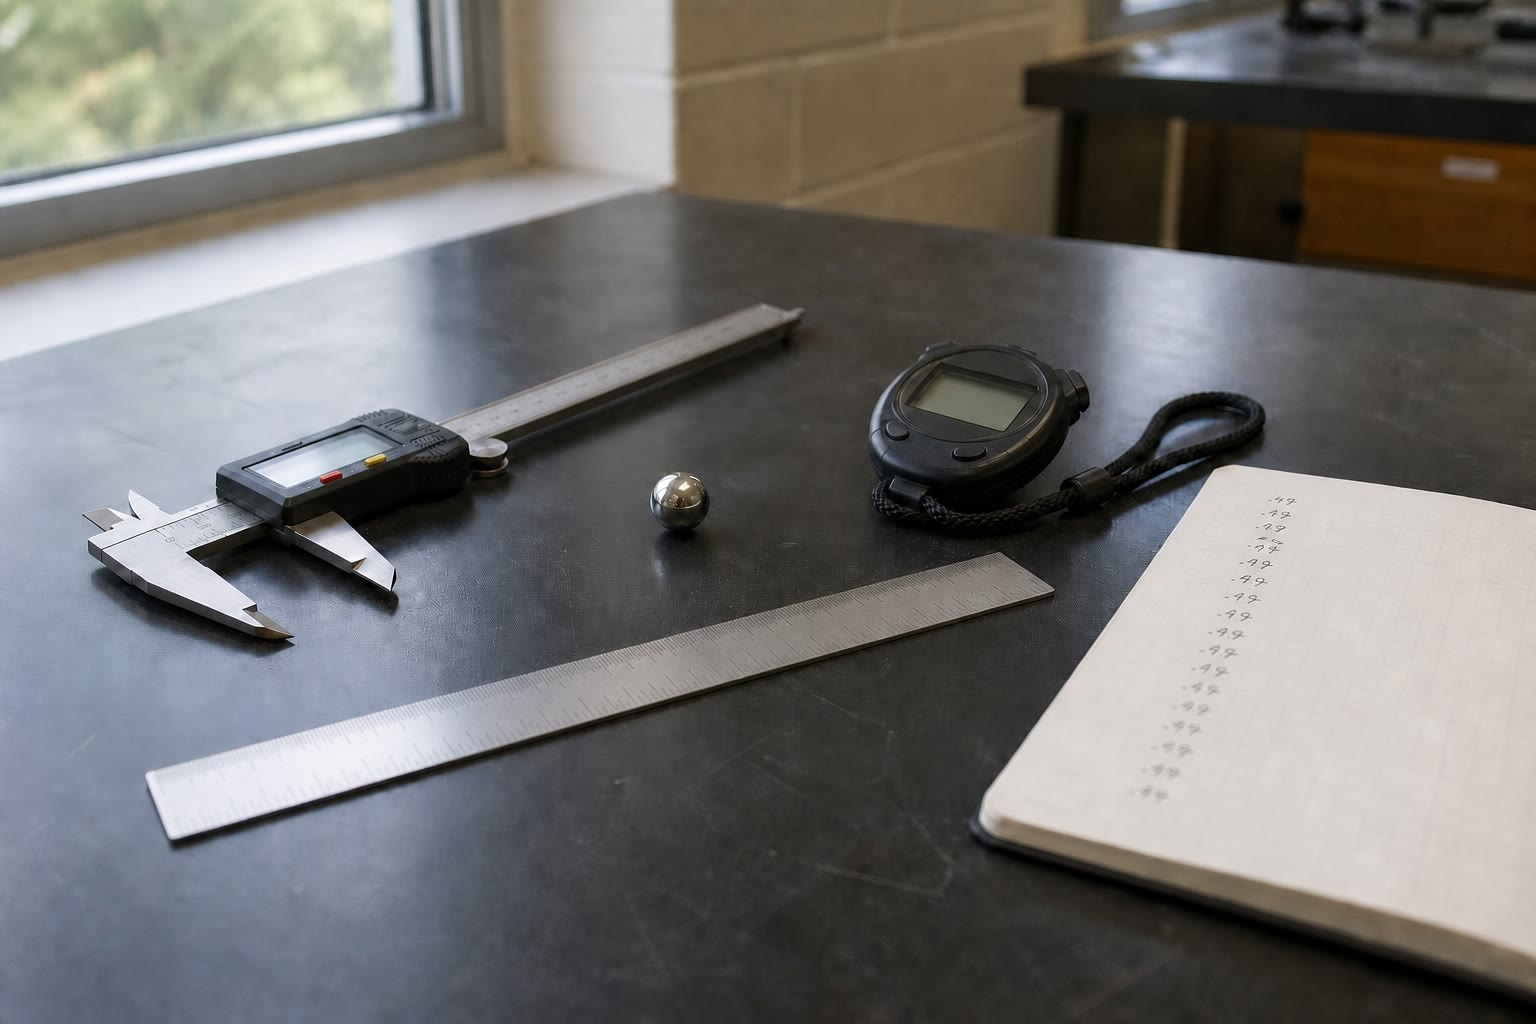
\includegraphics[width=0.60\linewidth]{images/book3/ai/b3-01-lab-bench-measuring.jpg}

{\small Bahan mentah bab ini: sebuah jangka sorong, sebuah stopwatch, sebuah bola, sebuah mistar, dan sekolom pembacaan berulang yang tak pernah benar-benar sama.}
\end{omfigure}

\section{Soal: Mengukur $g$ dengan sebuah bandul}

\begin{problem}[{Soal akhir pekan --- seutas tali, sebuah bandulan, sebuah
stopwatch dan sebuah pita ukur: seberapa baik meja dapur dapat mengukur
medan gravitasi Bumi, dan mana di antara empat angkanya yang lemah}]
\label{pb:b1:units-dimensions:1}
Sebuah bandul adalah bola baja yang digantung pada titik tetap dengan
tali ringan; ayunan kecilnya berperiode $\tau = 2\pi\sqrt{\ell/g}$
dengan $\ell$ jarak dari titik gantung ke pusat bolanya. Tujuannya
sebuah nilai $g$ dengan ketidakpastian yang dapat dipertanggungjawabkan.

\medskip
\noindent\textbf{Bagian I --- Modelnya.}
\begin{enumerate}
  \item Periksalah kehomogenan $\tau = 2\pi\sqrt{\ell/g}$.
  \item Bolanya bermassa $m$. Tunjukkan dengan \omterm{def:b1:units-dimensions:dimension}{dimensi} saja bahwa
        periodenya tidak mungkin bergantung pada $m$ jika ia hanya
        bergantung pada $\ell$, $g$ dan $m$.
  \item Periodenya juga bergantung, sedikit, pada amplitudo $\theta_0$
        ayunannya. Mengapa analisis \omterm{def:b1:units-dimensions:dimension}{dimensi} mengizinkan hal ini, dan apa
        yang harus dilakukan secara eksperimental agar rumusnya berlaku?
  \item Nyatakan $g$ sebagai fungsi $\ell$ dan $\tau$.
\end{enumerate}

\medskip
\noindent\textbf{Bagian II --- Mengukur panjangnya.}
Pita ukurnya berskala milimeter; talinya sepanjang
\qty{99.0}{cm} dari gantungan sampai puncak bolanya, diameter bolanya
\qty{2.00}{cm}, keduanya dibaca satu kali.
\begin{enumerate}[resume]
  \item Hitunglah $\ell$.
  \item Evaluasilah ketidakpastian tipe B sebuah pembacaan tunggal pada
        pita ukurnya.
  \item Menentukan letak titik gantung dan pusat bolanya menambahkan
        taksiran galat yang mungkin sebesar $\pm\qty{5}{mm}$ (seragam).
        Gabungkan dengan butir sebelumnya menjadi $u(\ell)$, lalu
        berikan ketidakpastian nisbinya $u(\ell)/\ell$.
\end{enumerate}

\medskip
\noindent\textbf{Bagian III --- Mengukur periodenya.}
Untuk mengurangi pengaruh waktu reaksi, orang mencatat waktu sepuluh
periode. Delapan pencatatan semacam itu, dalam sekon: $20.12$, $20.05$,
$20.18$, $20.09$, $20.15$, $20.02$, $20.11$, $20.08$.
\begin{enumerate}[resume]
  \item Mengapa mencatat sepuluh periode dan bukan satu? Mengapa
        mengulangi pencatatannya delapan kali?
  \item Hitunglah rata-rata $\overline{t_{10}}$ dan simpangan baku
        eksperimen $s$ kedelapan pencatatan itu.
  \item Simpulkan \omterm{def:b1:units-dimensions:uncertainty}{ketidakpastian baku} rata-ratanya, lalu periodenya
        $\tau$ dan ketidakpastiannya $u(\tau)$.
  \item Bandingkan $u(\tau)/\tau$ dengan $u(\ell)/\ell$.
\end{enumerate}

\medskip
\noindent\textbf{Bagian IV --- Hasilnya dan titik lemahnya.}
\begin{enumerate}[resume]
  \item Hitunglah $g$.
  \item Tuliskan $u(g)/g$ dalam $u(\ell)/\ell$ dan $u(\tau)/\tau$, lalu
        hitunglah.
  \item Tuliskan hasilnya dalam bentuk baku.
  \item Bandingkan dengan nilai acuan $\qty{9.81}{m/s^2}$ melalui
        \omterm{def:b1:units-dimensions:zscore}{simpangan ternormalisasi}. Kesimpulannya?
  \item Manakah di antara kedua besaran terukur itu yang membatasi
        ketelitian $g$? Usulkan dua perbaikan yang konkret dan katakan
        seberapa besar masing-masing akan menurunkan ketidakpastian
        nisbinya.
  \item Andaikan, karena penjajaran yang ceroboh, setiap panjang
        ditaksir terlalu besar sebanyak \qty{5}{mm}. Apakah hal ini
        sudah tercakup dalam anggaran ketidakpastiannya? Nama apa yang
        disandang galat semacam ini, dan bagaimana mendeteksinya?
\end{enumerate}

\medskip
\noindent\textbf{Bagian V --- Lima panjang dan sebuah garis lurus.}
Percobaannya diulang untuk $\ell = 0.400$, $0.600$, $0.800$,
$1.000$ dan \qty{1.200}{m}, memberi $\tau^2 = 1.62$, $2.41$, $3.25$,
$4.04$ dan \qty{4.84}{s^2}, masing-masing dengan $u(\tau^2) \approx 1\%$.
\begin{enumerate}[resume]
  \item Mengapa menggambarkan $\tau^2$ terhadap $\ell$ dan bukan $\tau$
        terhadap $\ell$?
  \item Hitunglah $\bar\ell$ dan $\overline{\tau^2}$.
  \item Hitunglah kemiringan \omterm{prop:b1:units-dimensions:regression}{kuadrat terkecil} $a$ dan perpotongan $b$.
  \item Simpulkan $g$ dari kemiringannya.
  \item Tafsirkan perpotongannya: apa yang akan disingkapkan oleh $b$
        yang jelas tak nol?
  \item Pencocokan oleh komputer melaporkan $u(a) = \qty{0.05}{s^2/m}$.
        Simpulkan $u(g)$ lalu tuliskan hasilnya.
  \item Bandingkan hasil panjang tunggal Bagian IV dengan hasil ini
        melalui \omterm{def:b1:units-dimensions:zscore}{simpangan ternormalisasi}.
  \item Seorang mahasiswa mengusulkan untuk mengukur sebagai gantinya
        satu ayunan bandul sepanjang \qty{10}{m} di sebuah tangga
        dengan pita ukur dan stopwatch yang sama. Taksirlah
        ketidakpastian nisbi $g$ yang akan diberikannya, lalu
        simpulkan strategi terbaiknya.
\end{enumerate}
\end{problem}
